\documentclass[a4paper,11pt]{article}

\usepackage[utf8]{inputenc}
\usepackage[T1]{fontenc}
\usepackage[english]{babel}
\usepackage[margin=2.2cm]{geometry}
\usepackage{amsmath,amssymb}
\usepackage{graphicx}
\usepackage{booktabs}
\usepackage{caption}
\usepackage[colorlinks=true,linkcolor=blue,citecolor=blue,urlcolor=blue]{hyperref}

\graphicspath{{../results/}}

\newcommand{\bx}{\boldsymbol{x}}
\newcommand{\by}{\boldsymbol{y}}
\newcommand{\bX}{\boldsymbol{X}}
\newcommand{\bth}{\boldsymbol{\theta}}
\newcommand{\beps}{\boldsymbol{\varepsilon}}

\title{Regression analysis, resampling methods and gradient descent\\
for the Runge function}
\author{Anne Kristin Furu\\
\small Department of Physics, University of Oslo\\
\small \url{https://github.com/Annekfu/FYS-STK4155-Project1}}
\date{FYS-STK4155, fall 2026}

\begin{document}
\maketitle

\begin{abstract}
\noindent
We study ordinary least squares (OLS), Ridge and Lasso regression on Runge's
function $f(x)=1/(1+25x^2)$ on $[-1,1]$, fitted with polynomials up to degree
15 on $n=100$ noisy points. We assess the models with the bootstrap and with
$k$-fold cross-validation, and we replace the closed-form solutions by gradient
descent with momentum and the adaptive methods AdaGrad, RMSProp and Adam, both
with the full gradient and with minibatches. Our own solvers reproduce the
closed-form OLS and Ridge solutions, the analytical gradient matches automatic
differentiation to machine precision ($\sim 10^{-15}$), and our proximal Lasso
matches scikit-learn to $\sim 10^{-10}$. The bootstrap makes the bias--variance
tradeoff explicit: the variance rises steeply with the polynomial degree while
the bias stays low. Cross-validation selects the models cleanly, and OLS
(degree 12, CV MSE $\approx 0.019$) and Ridge ($\approx 0.021$) are essentially
tied, with Lasso a little higher ($\approx 0.027$). On this smooth,
low-dimensional problem the penalties buy little over a well-chosen OLS degree.
\end{abstract}

\section{Introduction}
Polynomial regression is the simplest setting in which the central tension of
supervised learning appears: a more flexible model fits the training data
better but generalises worse. Runge's function
\begin{equation}
f(x)=\frac{1}{1+25x^2}, \qquad x\in[-1,1],
\label{eq:runge}
\end{equation}
is a classic hard case for polynomial interpolation, with a sharp central peak
that low-degree polynomials cannot follow and high-degree polynomials
overfit. It is therefore a good testbed for regression and model selection.

In this project we (i) fit \eqref{eq:runge} with OLS and Ridge using our own
closed-form code; (ii) study the bias--variance tradeoff with the bootstrap and
select models with cross-validation; (iii) replace the closed form by gradient
descent, with the gradient computed both analytically and by automatic
differentiation, and extend it with momentum and the adaptive methods; (iv)
solve Lasso, which has no closed form, by proximal gradient descent; and (v)
compare OLS, Ridge and Lasso with cross-validation. Throughout we work with
scaled data and a fixed random seed for reproducibility.

The report is organised as follows. Section~\ref{sec:theory} sets up the theory
and methods, including the derivation of the bias--variance decomposition.
Section~\ref{sec:code} describes the code and the validation tests.
Section~\ref{sec:results} presents and discusses the results part by part, and
Section~\ref{sec:conclusion} concludes.

\section{Theory and methods}
\label{sec:theory}

\subsection{Ordinary least squares}
We model the data as $\by=\bX\bth+\beps$ with independent noise
$\varepsilon_i\sim\mathcal{N}(0,\sigma^2)$ and a design matrix $\bX$ whose
columns are powers of $x$. OLS minimises the mean squared error
\begin{equation}
C(\bth)=\frac{1}{n}\lVert\bX\bth-\by\rVert_2^2,
\end{equation}
with the closed-form minimiser $\hat{\bth}=(\bX^T\bX)^{-1}\bX^T\by$. Assuming the
model is correct, the estimator is unbiased and has variance
\begin{equation}
\mathbb{E}[\hat{\bth}]=\bth,\qquad
\mathrm{Var}(\hat{\bth})=\sigma^2(\bX^T\bX)^{-1},
\label{eq:olsvar}
\end{equation}
so the diagonal of \eqref{eq:olsvar} gives a confidence interval for each
coefficient, with $\sigma^2$ estimated from the residuals as
$\hat{\sigma}^2=\lVert\by-\bX\hat{\bth}\rVert_2^2/(n-p)$. We solve the normal
equations through the singular value decomposition (SVD) rather than an explicit
inverse, for numerical stability. The quality of the fit is measured by the MSE
and by the $R^2$ score.

\subsection{Ridge regression and singular-value shrinkage}
Ridge adds an $\ell_2$ penalty, $C(\bth)=\frac1n\lVert\bX\bth-\by\rVert^2
+\lambda\lVert\bth\rVert^2$, with the closed form
\begin{equation}
\hat{\bth}_{\text{Ridge}}=(\bX^T\bX+n\lambda\boldsymbol{I})^{-1}\bX^T\by .
\end{equation}
The factor $n$ comes from the $1/n$ in the data term; scikit-learn omits it, so
its \texttt{alpha} equals $n\lambda$. Writing $\bX=U S V^T$, the Ridge
coefficient in singular direction $i$ is the OLS one multiplied by the filter
factor
\begin{equation}
f_i=\frac{s_i^2}{s_i^2+n\lambda},
\label{eq:filter}
\end{equation}
so directions with large singular values are kept and small-singular-value
directions are shrunk toward zero (Section 3.8 of \cite{HjorthJensen2026},
\cite{vanWieringen2021}). These small-singular-value directions are exactly the
ill-conditioned ones that make the OLS coefficients unstable.

\subsection{Lasso}
Lasso replaces the penalty by the $\ell_1$ norm, $\lambda\lVert\bth\rVert_1$,
which has no closed form and is not differentiable at $\theta_j=0$; its
subdifferential there is $[-1,1]$. We solve it by proximal gradient descent
(ISTA): a gradient step on the smooth data term followed by the soft
thresholding operator $S_t(z)=\mathrm{sign}(z)\max(|z|-t,0)$, the proximal
operator of the $\ell_1$ penalty, which drives coefficients exactly to zero and
so yields a sparse model.

\subsection{The bias--variance decomposition}
Assume the data are generated by $\by=f(\bx)+\beps$ with
$\beps\sim\mathcal{N}(0,\sigma^2)$, and let $\tilde{\by}$ be the prediction of a
model fitted on a random training set. Adding and subtracting
$\mathbb{E}[\tilde{\by}]$ inside the expected squared error and grouping the
terms as $y-\tilde{y}=(f-\mathbb{E}[\tilde{y}])+\varepsilon
+(\mathbb{E}[\tilde{y}]-\tilde{y})$, the three squares survive and the three
cross terms vanish, each by one assumption: zero-mean noise, $f$ non-stochastic,
and the independence of the test-point noise from the training set. The result
is
\begin{equation}
\mathbb{E}\!\left[(\by-\tilde{\by})^2\right]
=\underbrace{\frac1n\sum_i\bigl(f_i-\mathbb{E}[\tilde{y}_i]\bigr)^2}_{\text{Bias}^2}
+\underbrace{\frac1n\sum_i\mathrm{Var}(\tilde{y}_i)}_{\text{Variance}}
+\sigma^2 .
\label{eq:bv}
\end{equation}
The expectation runs over both the noise and the random training set. The bias
measures how far the average model is from the truth, the variance how much the
model moves between training sets, and $\sigma^2$ is the irreducible noise. When
the true $f$ is unknown we estimate the bias against the noisy test targets, so
the measured bias absorbs $\sigma^2$; the printed identity
$\text{error}=\text{bias}+\text{variance}$ then holds per point, with the bias an
upper estimate.

\subsection{Resampling}
The bootstrap estimates \eqref{eq:bv} by refitting the model on resamples of the
training set and reading off the mean, the spread and the error of the
predictions on a fixed test set. Cross-validation instead splits the data into
$k$ folds, using each fold once as the test set, and averages the test MSE. Any
scaling is fitted inside each fold, on the training folds only, so the held-out
fold stays unseen.

\subsection{Gradient descent and its extensions}
Gradient descent updates $\bth_{k+1}=\bth_k-\gamma\nabla C(\bth_k)$ with the
analytical gradient $\nabla C_{\text{OLS}}=\frac2n\bX^T(\bX\bth-\by)$. It
converges only for $\gamma<2/\lambda_{\max}$, where $\lambda_{\max}$ is the
largest eigenvalue of the Hessian $\frac2n\bX^T\bX$, is fastest at
$\gamma^\ast=2/(\lambda_{\max}+\lambda_{\min})$, and slows as the condition
number $\kappa=\lambda_{\max}/\lambda_{\min}$ grows. Momentum, AdaGrad, RMSProp
and Adam \cite{Kingma2015} accelerate or stabilise this. The adaptive methods
give each coordinate its own step $\gamma/\sqrt{v_j}$, so $\gamma$ becomes a
length in parameter space and cannot violate the stability bound. Stochastic
gradient descent replaces the full gradient by a minibatch gradient inside an
epoch loop; the minibatch gradient is unbiased with noise $\propto 1/\sqrt{M}$,
so at a constant learning rate the iterate plateaus, and a decaying schedule
$\gamma_t=t_0/(t+t_1)$ is needed to converge.

\subsection{Automatic differentiation}
Automatic differentiation applies the exact chain rule through the code; it is
neither symbolic nor a finite difference, so it carries no truncation error, and
in reverse mode a full gradient costs only two to three cost evaluations
\cite{Baydin2018,Jax2018}. We use it to check our analytical gradient.

\section{Code structure and validation}
\label{sec:code}
The code is organised in three folders: \texttt{code} (reusable modules and the
notebooks), \texttt{results} (figures) and \texttt{report}. The modules
separate the data generation, the three regression methods, the optimisers and
the resampling tools, and the five notebooks import them, one per pair of
project parts. All randomness uses the seed 2026.

Following the recommendation that a code be checked against known results, we
validate every component: our SVD and pseudoinverse OLS agree with each other
and with scikit-learn; the analytical gradient matches \texttt{jax.grad} to
about $10^{-15}$ for both OLS and Ridge; the Ridge closed form matches
scikit-learn once \texttt{alpha}$=n\lambda$; our proximal Lasso matches
scikit-learn to about $10^{-10}$; and our own $k$-fold reproduces the
scikit-learn cross-validation.

\section{Results and discussion}
\label{sec:results}

\subsection{OLS (part a)}
Figure~\ref{fig:a} shows the training and test MSE against the polynomial
degree. The training MSE falls monotonically toward the noise floor
$\sigma^2=0.01$, while the test MSE has a broad minimum around degrees 6--12 and
rises again at high degree as the model fits the noise. The coefficient norm
grows with the degree, the signature of variance. Scaling does not change the
OLS predictions, but it controls the conditioning: Figure~\ref{fig:acond} shows
that the condition number of $\bX^T\bX$ still reaches $\sim 10^{10}$ at degree 15
even after standardisation, because standardisation removes the difference in
column magnitudes but not the strong correlation between the polynomial columns.
More data pushes the overfitting to higher degree and lowers the test error.

\begin{figure}[htb]
\centering
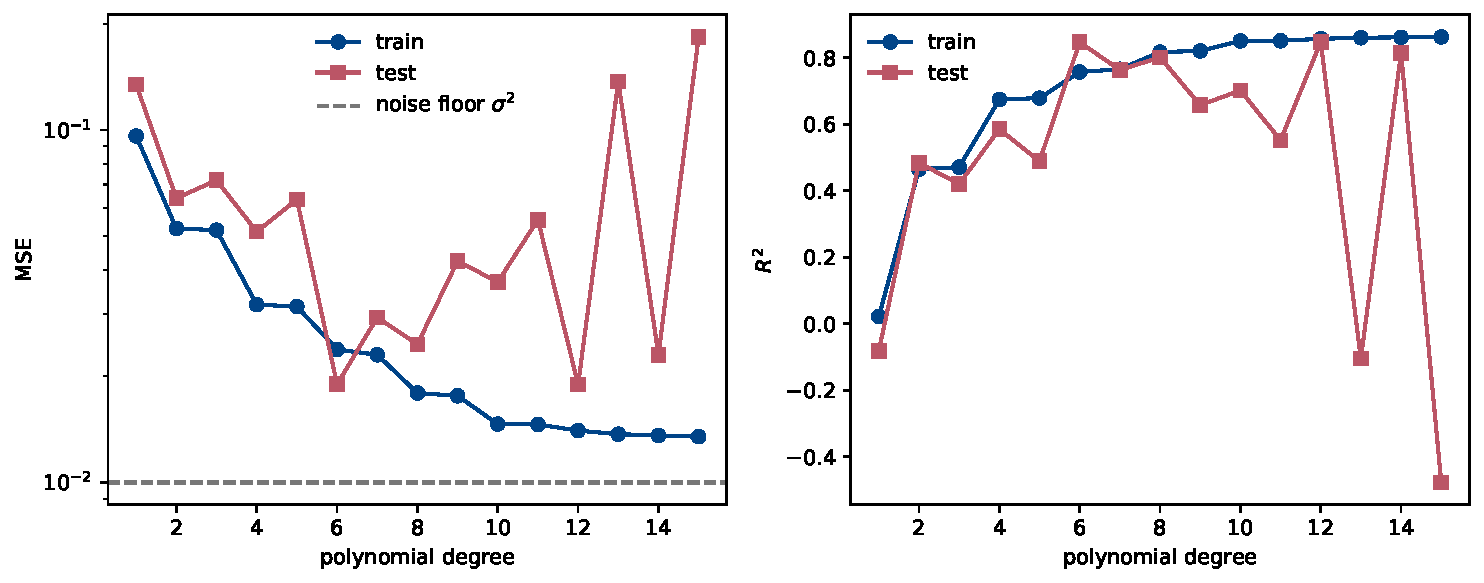
\includegraphics[width=\linewidth]{a_mse_r2.pdf}
\caption{OLS on Runge: training and test MSE (left) and $R^2$ (right) versus
polynomial degree. The dashed line is the noise floor $\sigma^2$.}
\label{fig:a}
\end{figure}

\begin{figure}[htb]
\centering
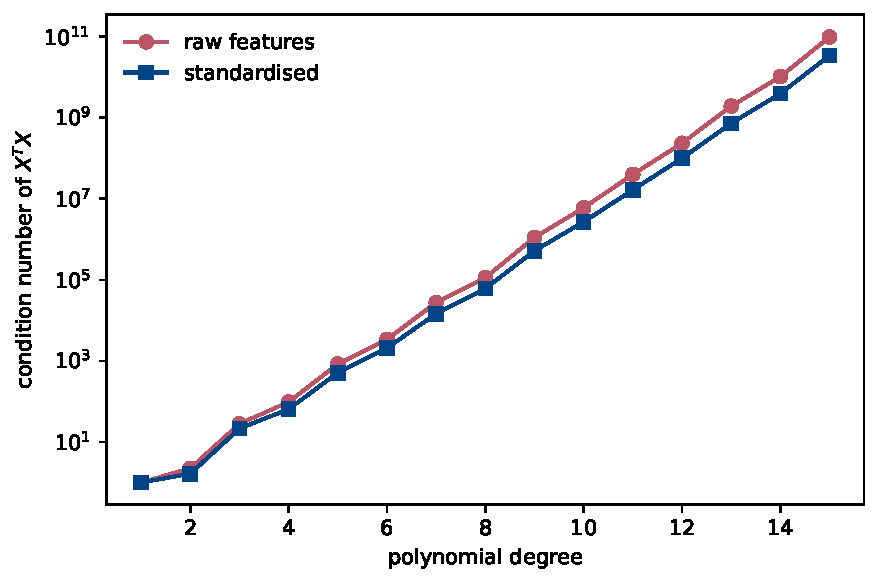
\includegraphics[width=0.6\linewidth]{a_conditioning.pdf}
\caption{Condition number of $\bX^T\bX$ versus degree, with and without
standardisation. Standardisation helps but does not remove the
ill-conditioning at high degree.}
\label{fig:acond}
\end{figure}

\subsection{Ridge (part b)}
A small penalty lowers the test error below OLS at high degree, while a large
penalty underfits. Figure~\ref{fig:bshrink} illustrates the mechanism through
the filter factors \eqref{eq:filter}: directions with a large singular value are
untouched, and small-singular-value directions are shrunk to zero. Ridge does
not change the model; it changes which directions the fit trusts, damping the
noisy directions that made the OLS coefficients blow up.

\begin{figure}[htb]
\centering
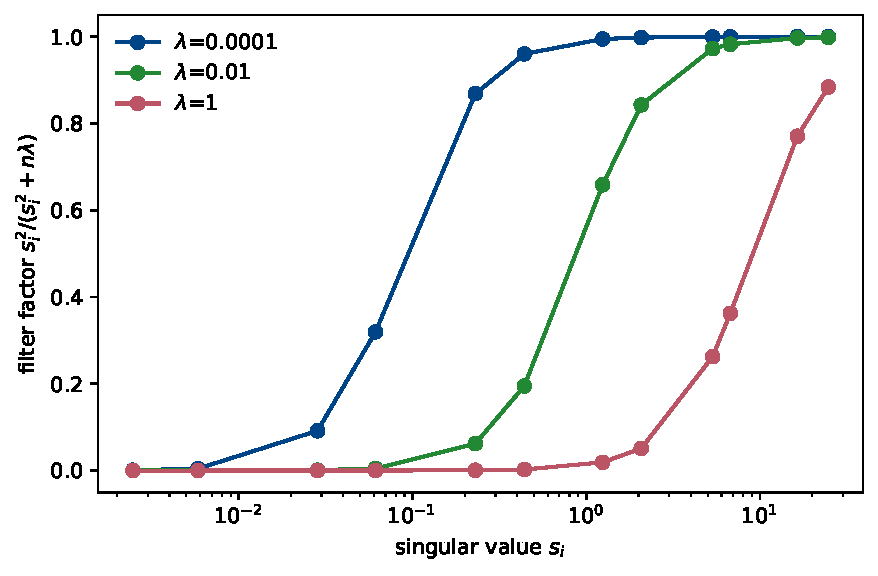
\includegraphics[width=0.6\linewidth]{b_shrinkage.pdf}
\caption{Ridge singular-value shrinkage: the filter factor
$s_i^2/(s_i^2+n\lambda)$ versus the singular value, for three penalties.}
\label{fig:bshrink}
\end{figure}

\subsection{Bias--variance with the bootstrap (part c)}
Figure~\ref{fig:c} decomposes the bootstrap test error into squared bias and
variance. The bias is low and roughly flat, the variance rises steeply with the
degree, and their sum gives the U-shaped test error. Repeating for
$n=40,100,400$ shows that more data lowers the variance and shifts the
overfitting to higher degree, while the bias barely moves: data reduces
variance, not bias.

\begin{figure}[htb]
\centering
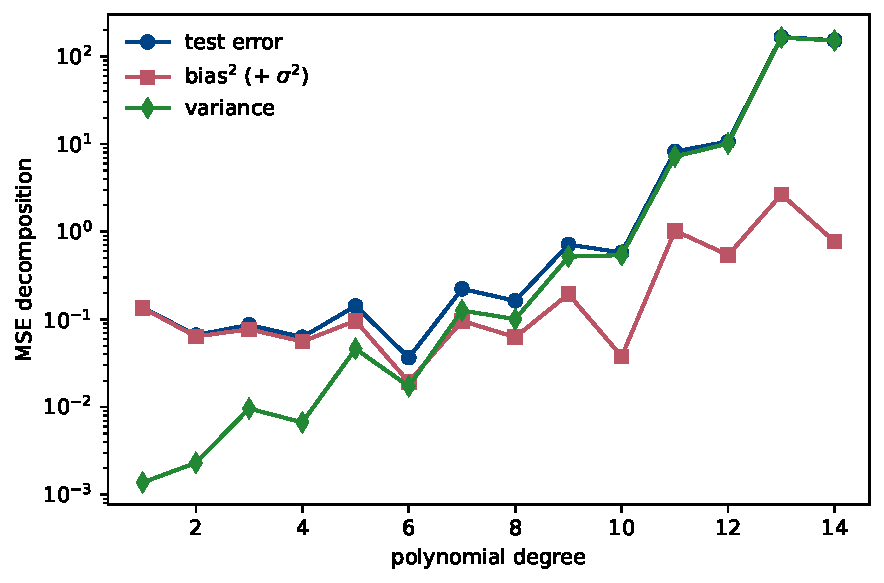
\includegraphics[width=0.55\linewidth]{c_bias_variance.pdf}
\caption{Bias--variance decomposition of the bootstrap test error versus degree
($n=100$).}
\label{fig:c}
\end{figure}

\subsection{Cross-validation (part d)}
Our own $k$-fold and the scikit-learn cross-validation agree closely, and both
track the bootstrap error and point to the same degree window
(Figure~\ref{fig:d}). At high degree the bootstrap error explodes while the
cross-validation stays flat, because a bootstrap resample can be nearly
rank-deficient, which destabilises OLS, whereas $k$-fold keeps distinct points.
The selected Ridge penalty is stable between $k=5$ and $k=10$.

\begin{figure}[htb]
\centering
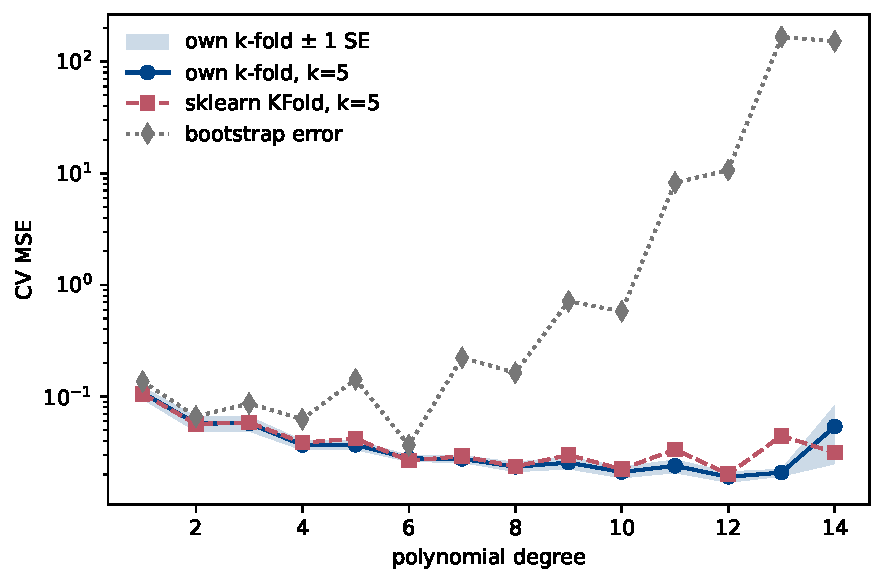
\includegraphics[width=0.55\linewidth]{d_cv_vs_bootstrap.pdf}
\caption{Cross-validated MSE (own $k$-fold and scikit-learn) versus degree,
compared with the bootstrap error.}
\label{fig:d}
\end{figure}

\subsection{Gradient descent and the adaptive methods (parts e, f)}
The analytical and automatic gradients agree to machine precision, so either can
drive the descent. Figure~\ref{fig:e} confirms the stability edge: just below
$2/\lambda_{\max}$ the iteration converges, just above it diverges, and
$\gamma^\ast$ is fastest. On the harder degree-6 problem ($\kappa\approx 2000$),
momentum and Adam reach the tolerance in about 1600 and 1300 iterations against
17000 for plain gradient descent (Figure~\ref{fig:f}); AdaGrad and RMSProp do
not reach it at a constant rate. Adam converges over the widest range of
learning rates and is the least sensitive to the choice.

\begin{figure}[htb]
\centering
\begin{minipage}{0.49\linewidth}
\centering
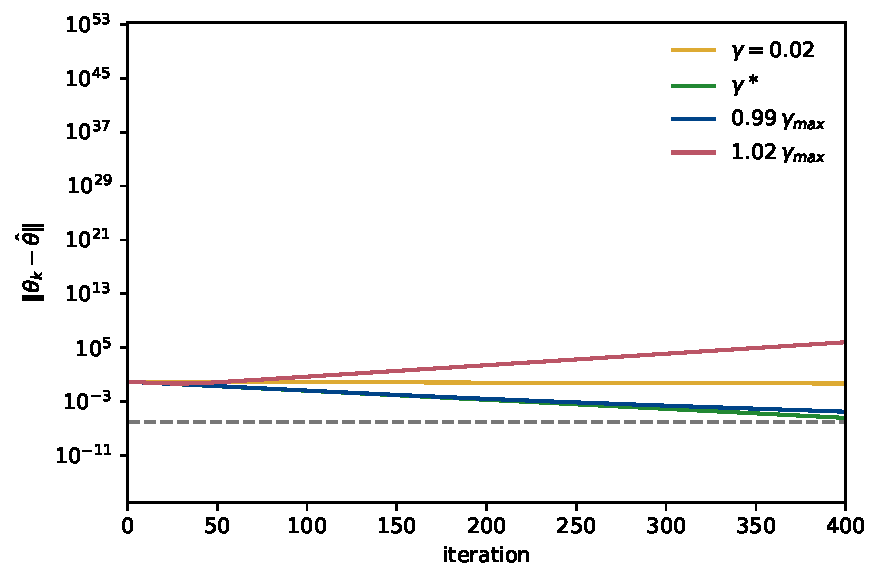
\includegraphics[width=\linewidth]{e_learning_rate.pdf}
\caption{Plain gradient descent for several learning rates (degree 4).}
\label{fig:e}
\end{minipage}\hfill
\begin{minipage}{0.49\linewidth}
\centering
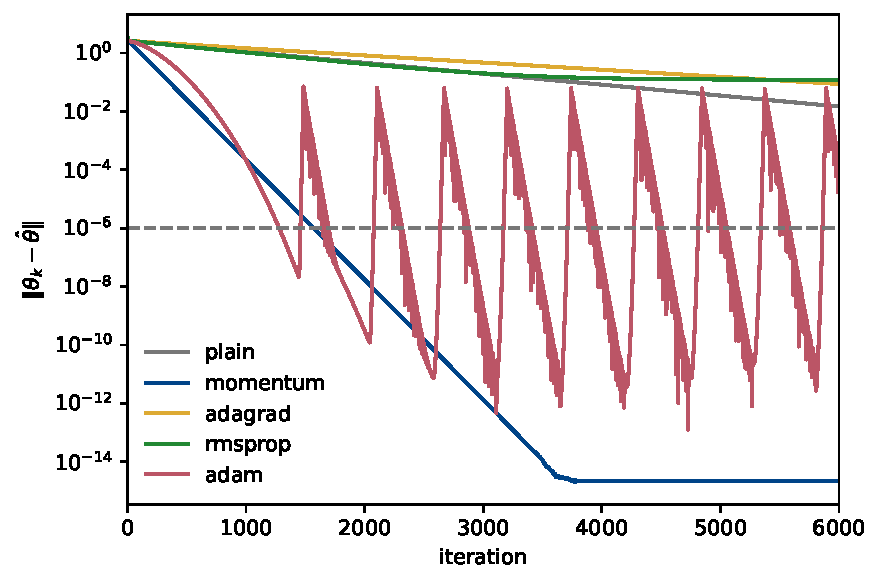
\includegraphics[width=\linewidth]{f_optimisers.pdf}
\caption{The five optimisers on the degree-6 problem.}
\label{fig:f}
\end{minipage}
\end{figure}

\subsection{Lasso (part g)}
JAX returns 1 for the derivative of $|\theta|$ at zero, a valid subgradient
since $1\in[-1,1]$; proximal gradient descent is the cleaner tool and sets
coefficients exactly to zero. Figure~\ref{fig:g} shows the key difference
between the penalties: Lasso removes coefficients one by one as $\lambda$ grows,
ending with a sparse model, while Ridge keeps all of them and only shrinks.

\begin{figure}[htb]
\centering
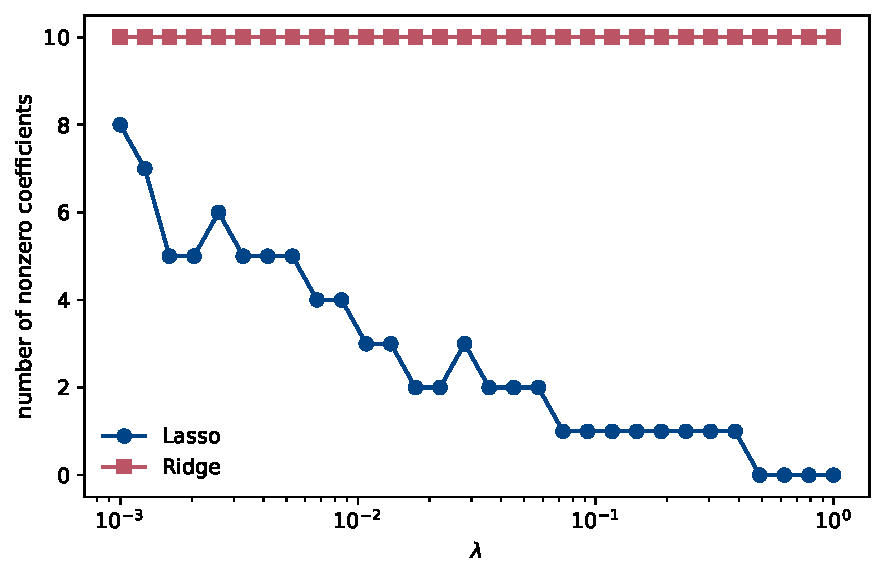
\includegraphics[width=0.55\linewidth]{g_sparsity.pdf}
\caption{Number of nonzero coefficients versus $\lambda$ for Lasso and Ridge
(degree 10).}
\label{fig:g}
\end{figure}

\subsection{Stochastic gradient descent (part h)}
On the well-conditioned degree-2 problem (Figure~\ref{fig:h}), full-batch
gradient descent converges geometrically to machine precision. Constant-rate
SGD does not converge; it plateaus at a height that scales with the learning
rate, because the iterate is a random walk in a noise cloud. A decaying schedule
shrinks that cloud and keeps descending. A single-point step can even diverge in
the ill-conditioned case, since it sees that one point's Hessian, which is why
Adam with minibatches is the safe default.

\begin{figure}[htb]
\centering
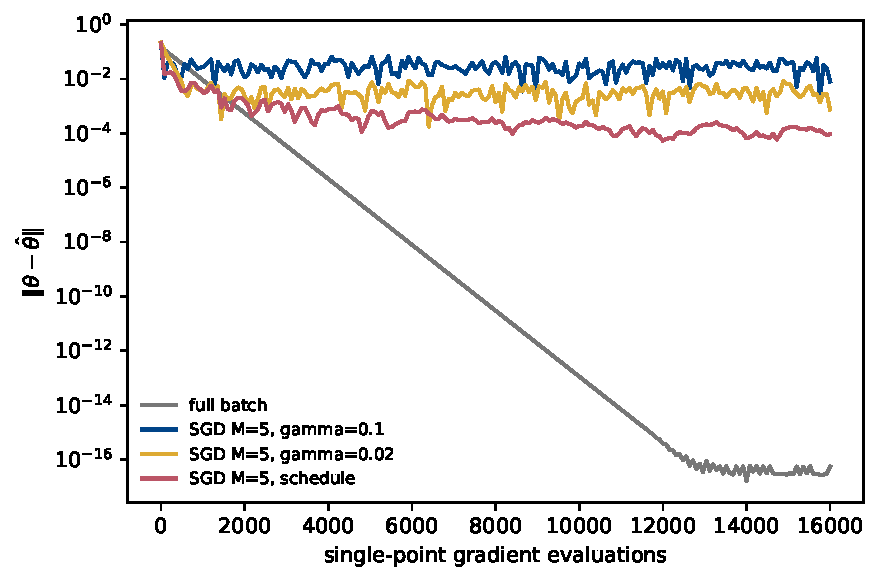
\includegraphics[width=0.55\linewidth]{h_sgd_vs_full.pdf}
\caption{SGD versus full-batch gradient descent (degree 2): constant learning
rates plateau, the schedule keeps descending.}
\label{fig:h}
\end{figure}

\subsection{Final comparison (part i)}
Selecting each method by 5-fold cross-validation on Runge gives OLS at degree 12
(CV MSE $\approx 0.019$), Ridge at degree 12 with a tiny penalty
($\approx 0.021$) and Lasso at degree 6 ($\approx 0.027$). OLS and Ridge are
essentially tied and Lasso is slightly higher; all three follow Runge's peak
(Figure~\ref{fig:i}). Read through \eqref{eq:bv}, OLS controls only the degree,
Ridge attacks the variance by shrinking the small-singular-value modes, and
Lasso attacks the variance and also cuts the effective complexity by zeroing
coefficients. On this smooth, low-dimensional problem with $n\gg p$ the
penalties buy little over a cross-validated OLS degree; the sparsity of Lasso
would pay off with many irrelevant features.

\begin{figure}[htb]
\centering
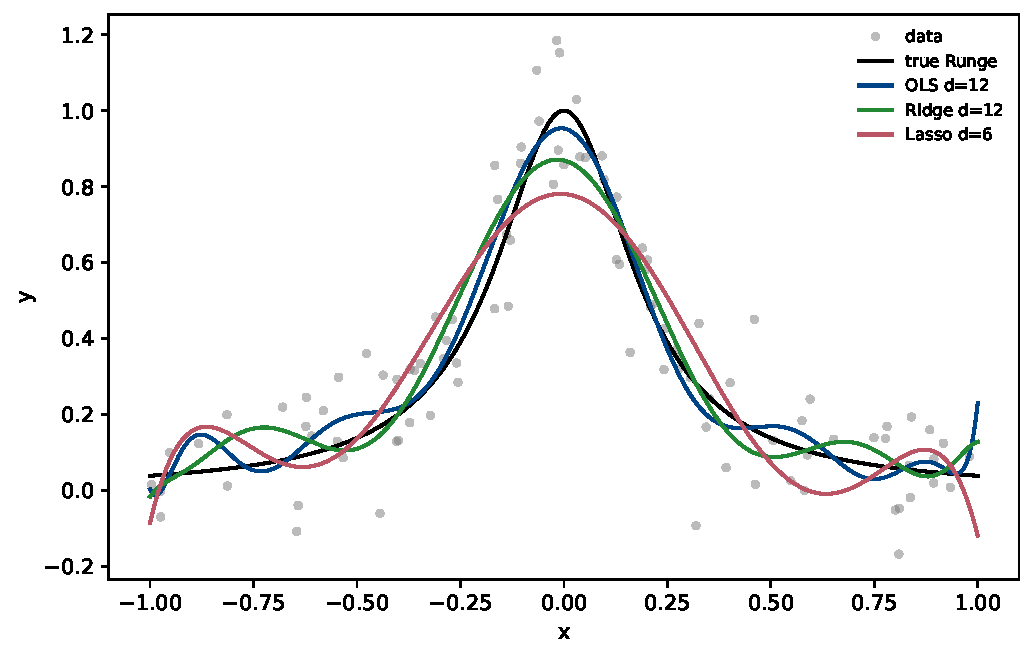
\includegraphics[width=0.6\linewidth]{i_fits.pdf}
\caption{The three cross-validated models refitted on all data, against the true
Runge function and the noisy sample.}
\label{fig:i}
\end{figure}

\section{Conclusion and perspectives}
\label{sec:conclusion}
We built and validated our own OLS, Ridge and Lasso solvers and a family of
gradient-descent optimisers, and applied them to Runge's function. The bootstrap
made the bias--variance tradeoff explicit, cross-validation selected the models
cleanly, and the gradient-descent study reproduced the closed-form solutions and
showed how the learning rate, the condition number and the choice of optimiser
interact. On this smooth one-dimensional problem OLS, Ridge and Lasso reach
almost the same cross-validated error, so regularisation is not decisive here;
its value would show on higher-dimensional or noisier data, or with many
irrelevant features, which would be a natural next step. A second extension is to
replace the linear model by a neural network, keeping the same optimisers and
the same cross-validation, where the convexity that made the closed form
available is lost and the gradient-descent machinery becomes essential.

\section*{Declaration on the use of AI tools}
This report and the accompanying code were developed with the assistance of a
large language model (Claude, Opus 4.8, from Anthropic). The model was used to
scope the project against the weekly exercises, to help structure and write the
Python modules and notebooks by porting the author's own weekly-exercise
solutions to the Runge dataset, to generate the figures, and to help draft this
report. All prompts and direction came from the author, who has reviewed and
verified every result, understands the methods, and is responsible for every
line of code and every claim in the report. The libraries used are cited in the
bibliography.

\bibliographystyle{plain}
\bibliography{references}

\end{document}
